\documentclass[12pt, a4paper,  BCOR=8.25mm, DIV=15]{scrartcl}\usepackage[]{graphicx}\usepackage[]{color}
%% maxwidth is the original width if it is less than linewidth
%% otherwise use linewidth (to make sure the graphics do not exceed the margin)
\makeatletter
\def\maxwidth{ %
  \ifdim\Gin@nat@width>\linewidth
    \linewidth
  \else
    \Gin@nat@width
  \fi
}
\makeatother

\definecolor{fgcolor}{rgb}{0.345, 0.345, 0.345}
\newcommand{\hlnum}[1]{\textcolor[rgb]{0.686,0.059,0.569}{#1}}%
\newcommand{\hlstr}[1]{\textcolor[rgb]{0.192,0.494,0.8}{#1}}%
\newcommand{\hlcom}[1]{\textcolor[rgb]{0.678,0.584,0.686}{\textit{#1}}}%
\newcommand{\hlopt}[1]{\textcolor[rgb]{0,0,0}{#1}}%
\newcommand{\hlstd}[1]{\textcolor[rgb]{0.345,0.345,0.345}{#1}}%
\newcommand{\hlkwa}[1]{\textcolor[rgb]{0.161,0.373,0.58}{\textbf{#1}}}%
\newcommand{\hlkwb}[1]{\textcolor[rgb]{0.69,0.353,0.396}{#1}}%
\newcommand{\hlkwc}[1]{\textcolor[rgb]{0.333,0.667,0.333}{#1}}%
\newcommand{\hlkwd}[1]{\textcolor[rgb]{0.737,0.353,0.396}{\textbf{#1}}}%
\let\hlipl\hlkwb

\usepackage{framed}
\makeatletter
\newenvironment{kframe}{%
 \def\at@end@of@kframe{}%
 \ifinner\ifhmode%
  \def\at@end@of@kframe{\end{minipage}}%
  \begin{minipage}{\columnwidth}%
 \fi\fi%
 \def\FrameCommand##1{\hskip\@totalleftmargin \hskip-\fboxsep
 \colorbox{shadecolor}{##1}\hskip-\fboxsep
     % There is no \\@totalrightmargin, so:
     \hskip-\linewidth \hskip-\@totalleftmargin \hskip\columnwidth}%
 \MakeFramed {\advance\hsize-\width
   \@totalleftmargin\z@ \linewidth\hsize
   \@setminipage}}%
 {\par\unskip\endMakeFramed%
 \at@end@of@kframe}
\makeatother

\definecolor{shadecolor}{rgb}{.97, .97, .97}
\definecolor{messagecolor}{rgb}{0, 0, 0}
\definecolor{warningcolor}{rgb}{1, 0, 1}
\definecolor{errorcolor}{rgb}{1, 0, 0}
\newenvironment{knitrout}{}{} % an empty environment to be redefined in TeX

\usepackage{alltt}
\usepackage[utf8]{inputenc}
\usepackage{newfloat}
\DeclareFloatingEnvironment[name={Supplementary Figure}]{suppfigure}

\newenvironment{itemizz}%
  {\begin{itemize}%
    \setlength{\itemsep}{2pt}%
    \setlength{\parskip}{2pt}}%
  {\end{itemize}}

\newcommand{\txtt}[1]{{\texttt{#1}}}
\IfFileExists{upquote.sty}{\usepackage{upquote}}{}
\begin{document}
%\VignetteEngine{knitr::knitr}
%\VignetteIndexEntry{Further methods (Set 12)}



\title{12: Further Methods}
\author{John H Maindonald}
\maketitle
\vspace{-0.5cm}

\begin{knitrout}
\definecolor{shadecolor}{rgb}{0.969, 0.969, 0.969}\color{fgcolor}\begin{kframe}
\begin{alltt}
\hlstd{doFigs} \hlkwb{<-} \hlnum{TRUE}
\end{alltt}
\end{kframe}
\end{knitrout}
\vspace{-0.5cm}

\begin{knitrout}
\definecolor{shadecolor}{rgb}{0.969, 0.969, 0.969}\color{fgcolor}\begin{kframe}
\begin{alltt}
\hlstd{fig12.1} \hlkwb{<-} \hlkwa{function}\hlstd{()\{}
\hlcom{## ---- smooth-ohms ----}
\hlcom{## Plot points}
\hlkwd{plot}\hlstd{(ohms} \hlopt{~} \hlstd{juice,} \hlkwc{data}\hlstd{=fruitohms)}
\hlcom{## Add smooth curve, using default}
\hlcom{## smoothing window}
\hlkwd{with}\hlstd{(fruitohms,}
     \hlkwd{lines}\hlstd{(}\hlkwd{lowess}\hlstd{(ohms} \hlopt{~} \hlstd{juice),} \hlkwc{col}\hlstd{=}\hlstr{"gray"}\hlstd{,} \hlkwc{lwd}\hlstd{=}\hlnum{2}\hlstd{))}
\hlstd{\}}
\end{alltt}
\end{kframe}
\end{knitrout}

\begin{figure}
\begin{knitrout}
\definecolor{shadecolor}{rgb}{0.969, 0.969, 0.969}\color{fgcolor}\begin{kframe}
\begin{alltt}
\hlstd{fig12.2A} \hlkwb{<-} \hlkwa{function}\hlstd{()\{}
    \hlkwa{if}\hlstd{(}\hlopt{!}\hlkwd{exists}\hlstd{(}\hlstr{"eyeAmpM.gam"}\hlstd{))}
\hlstd{eyeAmpM.gam} \hlkwb{<-} \hlstd{mgcv}\hlopt{::}\hlkwd{gam}\hlstd{(amp} \hlopt{~} \hlkwd{s}\hlstd{(x,y),} \hlkwc{data}\hlstd{=}\hlkwd{subset}\hlstd{(eyeAmp, Sex}\hlopt{==}\hlstr{"m"}\hlstd{))}
        \hlkwa{if}\hlstd{(}\hlopt{!}\hlkwd{exists}\hlstd{(}\hlstr{"eyeAmpF.gam"}\hlstd{))}
\hlstd{eyeAmpF.gam} \hlkwb{<-} \hlstd{mgcv}\hlopt{::}\hlkwd{gam}\hlstd{(amp} \hlopt{~} \hlkwd{s}\hlstd{(x,y),} \hlkwc{data}\hlstd{=}\hlkwd{subset}\hlstd{(eyeAmp, Sex}\hlopt{==}\hlstr{"f"}\hlstd{))}
\hlstd{lims} \hlkwb{<-} \hlkwd{range}\hlstd{(}\hlkwd{c}\hlstd{(}\hlkwd{predict}\hlstd{(eyeAmpF.gam),} \hlkwd{predict}\hlstd{(eyeAmpM.gam)))}
\hlstd{mgcv}\hlopt{::}\hlkwd{vis.gam}\hlstd{(eyeAmpM.gam,} \hlkwc{plot.type}\hlstd{=}\hlstr{'contour'}\hlstd{,} \hlkwc{color}\hlstd{=}\hlstr{"cm"}\hlstd{,} \hlkwc{zlim}\hlstd{=lims,} \hlkwc{main}\hlstd{=}\hlstr{""}\hlstd{)}
\hlstd{\}}
\hlstd{fig12.2B} \hlkwb{<-} \hlkwa{function}\hlstd{()\{}
    \hlkwa{if}\hlstd{(}\hlopt{!}\hlkwd{exists}\hlstd{(}\hlstr{"eyeAmpM.gam"}\hlstd{))}
    \hlstd{eyeAmpM.gam} \hlkwb{<-} \hlstd{mgcv}\hlopt{::}\hlkwd{gam}\hlstd{(amp} \hlopt{~} \hlkwd{s}\hlstd{(x,y),} \hlkwc{data}\hlstd{=}\hlkwd{subset}\hlstd{(eyeAmp, Sex}\hlopt{==}\hlstr{"m"}\hlstd{))}
    \hlkwa{if}\hlstd{(}\hlopt{!}\hlkwd{exists}\hlstd{(}\hlstr{"eyeAmpF.gam"}\hlstd{))}
    \hlstd{eyeAmpF.gam} \hlkwb{<-} \hlstd{mgcv}\hlopt{::}\hlkwd{gam}\hlstd{(amp} \hlopt{~} \hlkwd{s}\hlstd{(x,y),} \hlkwc{data}\hlstd{=}\hlkwd{subset}\hlstd{(eyeAmp, Sex}\hlopt{==}\hlstr{"f"}\hlstd{))}
\hlstd{lims} \hlkwb{<-} \hlkwd{range}\hlstd{(}\hlkwd{c}\hlstd{(}\hlkwd{predict}\hlstd{(eyeAmpF.gam),} \hlkwd{predict}\hlstd{(eyeAmpM.gam)))}
\hlstd{mgcv}\hlopt{::}\hlkwd{vis.gam}\hlstd{(eyeAmpF.gam,} \hlkwc{plot.type}\hlstd{=}\hlstr{'contour'}\hlstd{,} \hlkwc{color}\hlstd{=}\hlstr{"cm"}\hlstd{,} \hlkwc{zlim}\hlstd{=lims,} \hlkwc{main}\hlstd{=}\hlstr{""}\hlstd{)}
\hlstd{\}}
\hlstd{fig12.2} \hlkwb{<-} \hlkwa{function}\hlstd{()\{}
\hlkwd{print}\hlstd{(}\hlstr{"Run the separate figures fig12.2A() and fig12.2B()"}\hlstd{)}
\hlstd{\}}
\end{alltt}
\end{kframe}
\end{knitrout}
\end{figure}

\begin{knitrout}
\definecolor{shadecolor}{rgb}{0.969, 0.969, 0.969}\color{fgcolor}\begin{kframe}
\begin{alltt}
\hlstd{fig12.3} \hlkwb{<-} \hlkwa{function}\hlstd{()\{}
\hlcom{## ---- ant111b ----}
\hlcom{# ant111b is in DAAG}
\hlstd{Site} \hlkwb{<-} \hlkwd{with}\hlstd{(ant111b,} \hlkwd{reorder}\hlstd{(site, harvwt,}
                              \hlkwc{FUN}\hlstd{=mean))}
\hlkwd{stripplot}\hlstd{(Site} \hlopt{~} \hlstd{harvwt,} \hlkwc{data}\hlstd{=ant111b,}
          \hlkwc{scales}\hlstd{=}\hlkwd{list}\hlstd{(}\hlkwc{tck}\hlstd{=}\hlnum{0.5}\hlstd{),}
          \hlkwc{xlab}\hlstd{=}\hlstr{"Harvest weight of corn"}\hlstd{)}
\hlstd{\}}
\end{alltt}
\end{kframe}
\end{knitrout}

\begin{knitrout}
\definecolor{shadecolor}{rgb}{0.969, 0.969, 0.969}\color{fgcolor}\begin{kframe}
\begin{alltt}
\hlstd{fig12.4} \hlkwb{<-} \hlkwa{function}\hlstd{()\{}
\hlcom{## ---- Erie1 ----}
\hlkwd{plot}\hlstd{(Erie,} \hlkwc{xlab}\hlstd{=}\hlstr{""}\hlstd{,}
     \hlkwc{ylab}\hlstd{=}\hlstr{"Level (m)"}\hlstd{)}
\hlstd{\}}
\end{alltt}
\end{kframe}
\end{knitrout}

\begin{knitrout}
\definecolor{shadecolor}{rgb}{0.969, 0.969, 0.969}\color{fgcolor}\begin{kframe}
\begin{alltt}
\hlstd{fig12.5A} \hlkwb{<-} \hlkwa{function}\hlstd{()\{}
\hlcom{## ---- lagErie ----}
\hlcom{## Panel A}
\hlkwd{lag.plot}\hlstd{(Erie,} \hlkwc{lags}\hlstd{=}\hlnum{3}\hlstd{,}
         \hlkwc{do.lines}\hlstd{=}\hlnum{FALSE}\hlstd{,}
         \hlkwc{layout}\hlstd{=}\hlkwd{c}\hlstd{(}\hlnum{1}\hlstd{,}\hlnum{3}\hlstd{),}
         \hlkwc{main}\hlstd{=}\hlstr{"  "}\hlstd{)}
\hlkwd{mtext}\hlstd{(}\hlkwc{side}\hlstd{=}\hlnum{3}\hlstd{,} \hlkwc{line}\hlstd{=}\hlnum{2}\hlstd{,} \hlkwc{adj}\hlstd{=}\hlnum{0}\hlstd{,}
      \hlstr{"A: Lag plots, at lags of 1, 2 and 3"}\hlstd{)}
\hlstd{\}}
\hlstd{fig12.5B} \hlkwb{<-} \hlkwa{function}\hlstd{()\{}
\hlcom{## ---- acfErie ----}
\hlcom{## Panel B}
\hlkwd{acf}\hlstd{(Erie,} \hlkwc{main}\hlstd{=}\hlstr{""}\hlstd{)}
\hlkwd{mtext}\hlstd{(}\hlkwc{side}\hlstd{=}\hlnum{3}\hlstd{,} \hlkwc{line}\hlstd{=}\hlnum{1}\hlstd{,} \hlkwc{adj}\hlstd{=}\hlnum{0}\hlstd{,} \hlkwc{cex}\hlstd{=}\hlnum{1.25}\hlstd{,}
      \hlstr{"B: Autocorrelation function"}\hlstd{)}
\hlstd{\}}
\hlstd{fig12.5} \hlkwb{<-} \hlkwa{function}\hlstd{()\{}
\hlstr{"Run the separate functions fig12.5A() and fig12.5B()."}
\hlstd{\}}
\end{alltt}
\end{kframe}
\end{knitrout}

\begin{knitrout}
\definecolor{shadecolor}{rgb}{0.969, 0.969, 0.969}\color{fgcolor}\begin{kframe}
\begin{alltt}
\hlstd{fig12.6} \hlkwb{<-} \hlkwa{function}\hlstd{()\{}
\hlcom{## ---- gamErie ----}
\hlstd{df} \hlkwb{<-}  \hlkwd{data.frame}\hlstd{(}
  \hlkwc{height}\hlstd{=}\hlkwd{as.vector}\hlstd{(Erie),}
  \hlkwc{year}\hlstd{=}\hlkwd{time}\hlstd{(Erie))}
\hlstd{obj} \hlkwb{<-} \hlstd{mgcv}\hlopt{::}\hlkwd{gam}\hlstd{(height} \hlopt{~} \hlkwd{s}\hlstd{(year),} \hlkwc{data}\hlstd{=df)}
\hlkwd{plot}\hlstd{(obj,}
     \hlkwc{shift}\hlstd{=}\hlkwd{mean}\hlstd{(df}\hlopt{$}\hlstd{height),}
     \hlkwc{residuals}\hlstd{=}\hlnum{TRUE}\hlstd{,} \hlkwc{pch}\hlstd{=}\hlnum{1}\hlstd{,}
     \hlkwc{xlab}\hlstd{=}\hlstr{""}\hlstd{,}
     \hlkwc{ylab}\hlstd{=}\hlstr{"Height of lake"}\hlstd{)}
\hlstd{\}}
\end{alltt}
\end{kframe}
\end{knitrout}

\begin{knitrout}
\definecolor{shadecolor}{rgb}{0.969, 0.969, 0.969}\color{fgcolor}\begin{kframe}
\begin{alltt}
\hlstd{fig12.7} \hlkwb{<-} \hlkwa{function}\hlstd{()\{}
\hlcom{## ---- arima-sim ----}
\hlkwa{for} \hlstd{(i} \hlkwa{in} \hlnum{1}\hlopt{:}\hlnum{6}\hlstd{)\{}
\hlstd{ysim} \hlkwb{<-} \hlkwd{arima.sim}\hlstd{(}\hlkwd{list}\hlstd{(}\hlkwc{ar}\hlstd{=}\hlnum{0.85}\hlstd{),}
                  \hlkwc{n}\hlstd{=}\hlnum{200}\hlstd{)}
\hlstd{df} \hlkwb{<-} \hlkwd{data.frame}\hlstd{(}\hlkwc{x}\hlstd{=}\hlnum{1}\hlopt{:}\hlnum{200}\hlstd{,}
                 \hlkwc{y}\hlstd{=ysim)}
\hlstd{df.gam} \hlkwb{<-} \hlstd{mgcv}\hlopt{::}\hlkwd{gam}\hlstd{(y} \hlopt{~} \hlkwd{s}\hlstd{(x),}
              \hlkwc{data}\hlstd{=df)}
\hlkwd{plot}\hlstd{(df.gam,}
     \hlkwc{ylab}\hlstd{=}\hlkwd{paste}\hlstd{(}\hlstr{"Sim"}\hlstd{, i),}
     \hlkwc{residuals}\hlstd{=}\hlnum{TRUE}\hlstd{)}
\hlstd{\}}
\hlstd{\}}
\end{alltt}
\end{kframe}
\end{knitrout}

\begin{knitrout}
\definecolor{shadecolor}{rgb}{0.969, 0.969, 0.969}\color{fgcolor}\begin{kframe}
\begin{alltt}
\hlstd{fig12.8} \hlkwb{<-} \hlkwa{function}\hlstd{()\{}
\hlcom{## ---- Erie-fcast ----}
\hlstd{erie.ar} \hlkwb{<-} \hlkwd{ar}\hlstd{(Erie,} \hlkwc{order.max}\hlstd{=}\hlnum{1}\hlstd{)}
\hlstd{fc} \hlkwb{<-} \hlstd{forecast}\hlopt{::}\hlkwd{forecast}\hlstd{(erie.ar,} \hlkwc{h}\hlstd{=}\hlnum{15}\hlstd{)}
\hlkwd{plot}\hlstd{(fc,} \hlkwc{main}\hlstd{=}\hlstr{""}\hlstd{,}
     \hlkwc{ylab}\hlstd{=}\hlstr{"Lake level (m)"}\hlstd{)}
  \hlcom{# 15 time points ahead}
\hlstd{\}}
\end{alltt}
\end{kframe}
\end{knitrout}

\begin{knitrout}
\definecolor{shadecolor}{rgb}{0.969, 0.969, 0.969}\color{fgcolor}\begin{kframe}
\begin{alltt}
\hlstd{fig12.9} \hlkwb{<-} \hlkwa{function}\hlstd{()\{}
\hlcom{## ---- mdb-gam ----}
\hlstd{mdbRain.gam} \hlkwb{<-} \hlstd{mgcv}\hlopt{::}\hlkwd{gam}\hlstd{(mdbRain} \hlopt{~} \hlkwd{s}\hlstd{(Year)} \hlopt{+} \hlkwd{s}\hlstd{(SOI),}
                   \hlkwc{data}\hlstd{=bomregions)}
\hlkwd{plot}\hlstd{(mdbRain.gam,} \hlkwc{residuals}\hlstd{=}\hlnum{TRUE}\hlstd{,} \hlkwc{se}\hlstd{=}\hlnum{2}\hlstd{,} \hlkwc{pch}\hlstd{=}\hlnum{1}\hlstd{,}
     \hlkwc{cex}\hlstd{=}\hlnum{0.5}\hlstd{)}
\hlstd{\}}
\end{alltt}
\end{kframe}
\end{knitrout}

\begin{knitrout}
\definecolor{shadecolor}{rgb}{0.969, 0.969, 0.969}\color{fgcolor}\begin{kframe}
\begin{alltt}
\hlstd{fig12.10} \hlkwb{<-} \hlkwa{function}\hlstd{()\{}
\hlcom{## ---- ar1sims ----}
\hlstd{opar} \hlkwb{<-} \hlkwd{par}\hlstd{(}\hlkwc{mar}\hlstd{=}\hlkwd{c}\hlstd{(}\hlnum{2.1}\hlstd{,} \hlnum{3.1}\hlstd{,} \hlnum{0.25}\hlstd{,} \hlnum{1.1}\hlstd{),} \hlkwc{mgp}\hlstd{=}\hlkwd{c}\hlstd{(}\hlnum{2.25}\hlstd{,}\hlnum{0.5}\hlstd{,}\hlnum{0}\hlstd{))}
\hlstd{mdbRain.gam} \hlkwb{<-} \hlstd{mgcv}\hlopt{::}\hlkwd{gam}\hlstd{(mdbRain} \hlopt{~} \hlkwd{s}\hlstd{(Year)} \hlopt{+} \hlkwd{s}\hlstd{(SOI),}
                         \hlkwc{data}\hlstd{=bomregions)}
\hlstd{n} \hlkwb{<-}  \hlkwd{dim}\hlstd{(bomregions)[}\hlnum{1}\hlstd{]}
\hlkwd{acf}\hlstd{(}\hlkwd{resid}\hlstd{(mdbRain.gam),} \hlkwc{ylab}\hlstd{=}\hlstr{"MDB series"}\hlstd{)}
\hlkwa{for}\hlstd{(i} \hlkwa{in} \hlnum{1}\hlopt{:}\hlnum{5}\hlstd{)}\hlkwd{acf}\hlstd{(}\hlkwd{rnorm}\hlstd{(n),} \hlkwc{ylab}\hlstd{=}\hlkwd{paste}\hlstd{(}\hlstr{"Sim"}\hlstd{,i),}
                 \hlkwc{col}\hlstd{=}\hlstr{"gray40"}\hlstd{)}
\hlkwd{par}\hlstd{(opar)}
\hlstd{\}}
\end{alltt}
\end{kframe}
\end{knitrout}

\begin{knitrout}
\definecolor{shadecolor}{rgb}{0.969, 0.969, 0.969}\color{fgcolor}\begin{kframe}
\begin{alltt}
\hlkwd{library}\hlstd{(DAAGviz,} \hlkwc{quietly} \hlstd{=} \hlnum{TRUE}\hlstd{)}
\end{alltt}
\end{kframe}
\end{knitrout}

\begin{knitrout}
\definecolor{shadecolor}{rgb}{0.969, 0.969, 0.969}\color{fgcolor}\begin{kframe}
\begin{alltt}
\hlkwa{if}\hlstd{(}\hlopt{!}\hlkwd{requireNamespace}\hlstd{(}\hlstr{'gamclass'}\hlstd{,} \hlkwc{quietly}\hlstd{=}\hlnum{TRUE}\hlstd{))}\hlkwd{print}\hlstd{(}\hlstr{'gamclass must be installed'}\hlstd{)}
\hlstd{fromDate} \hlkwb{<-} \hlkwd{as.Date}\hlstd{(}\hlstr{"2006-01-01"}\hlstd{)}
\hlstd{dfDay06} \hlkwb{<-} \hlstd{gamclass}\hlopt{::}\hlkwd{eventCounts}\hlstd{(}\hlkwc{data}\hlstd{=gamclass}\hlopt{::}\hlstd{airAccs,} \hlkwc{dateCol}\hlstd{=}\hlstr{"Date"}\hlstd{,}
                       \hlkwc{from}\hlstd{= fromDate,} \hlkwc{by}\hlstd{=}\hlstr{'1 day'}\hlstd{,} \hlkwc{prefix}\hlstd{=}\hlstr{"num"}\hlstd{)}
\hlstd{dfDay06}\hlopt{$}\hlstd{day} \hlkwb{<-} \hlkwd{julian}\hlstd{(dfDay06}\hlopt{$}\hlstd{Date,} \hlkwc{origin}\hlstd{=fromDate)}
\hlstd{dfWeek06} \hlkwb{<-} \hlstd{gamclass}\hlopt{::}\hlkwd{eventCounts}\hlstd{(}\hlkwc{data}\hlstd{=gamclass}\hlopt{::}\hlstd{airAccs,} \hlkwc{dateCol}\hlstd{=}\hlstr{"Date"}\hlstd{,}
                        \hlkwc{from}\hlstd{=fromDate,}
                        \hlkwc{by}\hlstd{=}\hlstr{'1 week'}\hlstd{,} \hlkwc{prefix}\hlstd{=}\hlstr{"num"}\hlstd{)}
\hlstd{dfWeek06}\hlopt{$}\hlstd{day} \hlkwb{<-} \hlkwd{julian}\hlstd{(dfWeek06}\hlopt{$}\hlstd{Date,} \hlkwc{origin}\hlstd{=fromDate)}
\hlstd{year} \hlkwb{<-} \hlkwd{seq}\hlstd{(}\hlkwc{from}\hlstd{=fromDate,} \hlkwc{to}\hlstd{=}\hlkwd{max}\hlstd{(dfDay06}\hlopt{$}\hlstd{Date),} \hlkwc{by}\hlstd{=}\hlstr{"1 year"}\hlstd{)}
\hlstd{atyear}\hlkwb{=}\hlkwd{julian}\hlstd{(year,} \hlkwc{origin}\hlstd{=fromDate)}
\end{alltt}
\end{kframe}
\end{knitrout}

\begin{knitrout}
\definecolor{shadecolor}{rgb}{0.969, 0.969, 0.969}\color{fgcolor}\begin{kframe}
\begin{alltt}
\hlstd{fig12.11A} \hlkwb{<-} \hlkwa{function}\hlstd{()\{}
  \hlkwa{if}\hlstd{(}\hlopt{!}\hlkwd{exists}\hlstd{(}\hlstr{'dfday06'}\hlstd{))\{}
    \hlkwd{print}\hlstd{(}\hlkwd{paste}\hlstd{(}\hlstr{"Unable to plot graph."}\hlstd{,}
                \hlstr{"Ensure package 'gamclass' is installed."}\hlstd{))}
    \hlkwd{return}\hlstd{()}
  \hlstd{\}}
\hlstd{dfDay06.gam} \hlkwb{<-}
  \hlstd{mgcv}\hlopt{::}\hlkwd{gam}\hlstd{(}\hlkwc{formula} \hlstd{= num} \hlopt{~} \hlkwd{s}\hlstd{(day,} \hlkwc{k}\hlstd{=}\hlnum{200}\hlstd{),} \hlkwc{family} \hlstd{= quasipoisson,}
      \hlkwc{data} \hlstd{= dfDay06)}
\hlstd{av} \hlkwb{<-} \hlkwd{mean}\hlstd{(}\hlkwd{predict}\hlstd{(dfDay06.gam))}
\hlkwd{plot}\hlstd{(dfDay06.gam,} \hlkwc{xaxt}\hlstd{=}\hlstr{"n"}\hlstd{,} \hlkwc{shift}\hlstd{=av,} \hlkwc{trans}\hlstd{=exp,} \hlkwc{rug}\hlstd{=}\hlnum{FALSE}\hlstd{,} \hlkwc{xlab}\hlstd{=}\hlstr{""}\hlstd{,}
     \hlkwc{ylab}\hlstd{=}\hlstr{"Estimated rate per day"}\hlstd{)}
\hlkwd{axis}\hlstd{(}\hlnum{1}\hlstd{,} \hlkwc{at}\hlstd{=atyear,} \hlkwc{labels}\hlstd{=}\hlkwd{format}\hlstd{(year,} \hlstr{"%Y"}\hlstd{))}
\hlkwd{mtext}\hlstd{(}\hlkwc{side}\hlstd{=}\hlnum{3}\hlstd{,} \hlkwc{line}\hlstd{=}\hlnum{0.75}\hlstd{,} \hlstr{"A: Events per day, vs date"}\hlstd{,} \hlkwc{adj}\hlstd{=}\hlnum{0}\hlstd{)}
\hlstd{\}}
\hlstd{fig12.11B} \hlkwb{<-} \hlkwa{function}\hlstd{()\{}
\hlstd{dfWeek06.gam} \hlkwb{<-} \hlstd{mgcv}\hlopt{::}\hlkwd{gam}\hlstd{(num}\hlopt{~}\hlkwd{s}\hlstd{(day,} \hlkwc{k}\hlstd{=}\hlnum{200}\hlstd{),} \hlkwc{data}\hlstd{=dfWeek06,} \hlkwc{family}\hlstd{=quasipoisson)}
\hlstd{av} \hlkwb{<-} \hlkwd{mean}\hlstd{(}\hlkwd{predict}\hlstd{(dfWeek06.gam))}
\hlkwd{plot}\hlstd{(dfWeek06.gam,} \hlkwc{xaxt}\hlstd{=}\hlstr{"n"}\hlstd{,} \hlkwc{shift}\hlstd{=av,} \hlkwc{trans}\hlstd{=exp,} \hlkwc{rug}\hlstd{=}\hlnum{FALSE}\hlstd{,} \hlkwc{xlab}\hlstd{=}\hlstr{""}\hlstd{,}
      \hlkwc{ylab}\hlstd{=}\hlstr{"Estimated rate per week"}\hlstd{)}
\hlkwd{axis}\hlstd{(}\hlnum{1}\hlstd{,} \hlkwc{at}\hlstd{=atyear,} \hlkwc{labels}\hlstd{=}\hlkwd{format}\hlstd{(year,} \hlstr{"%Y"}\hlstd{))}
\hlkwd{mtext}\hlstd{(}\hlkwc{side}\hlstd{=}\hlnum{3}\hlstd{,} \hlkwc{line}\hlstd{=}\hlnum{0.75}\hlstd{,} \hlstr{"B: Events per week, vs date"}\hlstd{,} \hlkwc{adj}\hlstd{=}\hlnum{0}\hlstd{)}
\hlstd{\}}
\hlstd{fig12.11} \hlkwb{<-} \hlkwa{function}\hlstd{()\{}
    \hlstr{"Run the separate functions fig12.10A() & fig12.10B()"}
\hlstd{\}}
\end{alltt}
\end{kframe}
\end{knitrout}

\begin{knitrout}
\definecolor{shadecolor}{rgb}{0.969, 0.969, 0.969}\color{fgcolor}\begin{kframe}
\begin{alltt}
\hlstd{fig12.12} \hlkwb{<-} \hlkwa{function}\hlstd{()\{}
\hlcom{## ---- fgl-scores2D ----}
\hlstd{scores} \hlkwb{<-} \hlkwd{predict}\hlstd{(fgl.lda)}\hlopt{$}\hlstd{x}
\hlkwd{xyplot}\hlstd{(scores[,}\hlnum{2}\hlstd{]} \hlopt{~} \hlstd{scores[,}\hlnum{1}\hlstd{],} \hlkwc{groups}\hlstd{=fgl}\hlopt{$}\hlstd{type,}
       \hlkwc{xlab}\hlstd{=}\hlstr{"Discriminant 1"}\hlstd{,}
       \hlkwc{ylab}\hlstd{=}\hlstr{"Discriminant 2"}\hlstd{,}
       \hlkwc{aspect}\hlstd{=}\hlnum{1}\hlstd{,} \hlkwc{scales}\hlstd{=}\hlkwd{list}\hlstd{(}\hlkwc{tck}\hlstd{=}\hlnum{0.4}\hlstd{),}
       \hlkwc{auto.key}\hlstd{=}\hlkwd{list}\hlstd{(}\hlkwc{space}\hlstd{=}\hlstr{"right"}\hlstd{),}
       \hlkwc{par.settings}\hlstd{=}\hlkwd{simpleTheme}\hlstd{(}\hlkwc{alpha}\hlstd{=}\hlnum{0.6}\hlstd{,} \hlkwc{pch}\hlstd{=}\hlnum{1}\hlopt{:}\hlnum{6}\hlstd{))}
\hlstd{\}}
\end{alltt}
\end{kframe}
\end{knitrout}

\begin{knitrout}
\definecolor{shadecolor}{rgb}{0.969, 0.969, 0.969}\color{fgcolor}\begin{kframe}
\begin{alltt}
\hlcom{## ---- bronchit-first3 ----}
\hlcom{## ---- bronchit-rp ----}
\hlkwd{set.seed}\hlstd{(}\hlnum{47}\hlstd{)}   \hlcom{# Reproduce tree shown}
\hlstd{fig12.13} \hlkwb{<-} \hlkwa{function}\hlstd{()\{}
\hlcom{## ---- treefig ----}
\hlstd{opar} \hlkwb{<-} \hlkwd{par}\hlstd{(}\hlkwc{mar}\hlstd{=}\hlkwd{rep}\hlstd{(}\hlnum{1.1}\hlstd{,}\hlnum{4}\hlstd{))}
\hlkwa{if}\hlstd{(}\hlopt{!}\hlkwd{exists}\hlstd{(}\hlstr{'b.rpart'}\hlstd{))b.rpart} \hlkwb{<-} \hlkwd{rpart}\hlstd{(rfac} \hlopt{~} \hlstd{cig}\hlopt{+}\hlstd{poll,} \hlkwc{data}\hlstd{=bronchit)}
\hlkwd{plot}\hlstd{(b.rpart)}
\hlkwd{text}\hlstd{(b.rpart,} \hlkwc{xpd}\hlstd{=}\hlnum{TRUE}\hlstd{)}
\hlkwd{par}\hlstd{(opar)}
\hlstd{\}}
\end{alltt}
\end{kframe}
\end{knitrout}

\begin{knitrout}
\definecolor{shadecolor}{rgb}{0.969, 0.969, 0.969}\color{fgcolor}\begin{kframe}
\begin{alltt}
\hlstd{fig12.14} \hlkwb{<-} \hlkwa{function}\hlstd{()\{}
\hlcom{## ---- rf-x-bronchit ----}
\hlstd{opar} \hlkwb{<-} \hlkwd{par}\hlstd{(}\hlkwc{mar}\hlstd{=}\hlkwd{rep}\hlstd{(}\hlnum{2.1}\hlstd{,}\hlnum{4}\hlstd{))}
\hlkwd{set.seed}\hlstd{(}\hlnum{31}\hlstd{)}   \hlcom{# Reproduce the trees shown}
\hlstd{num} \hlkwb{<-} \hlnum{1}\hlopt{:}\hlkwd{nrow}\hlstd{(bronchit)}
\hlkwa{for}\hlstd{(i} \hlkwa{in} \hlnum{1}\hlopt{:}\hlnum{12}\hlstd{)\{}
  \hlstd{useobs} \hlkwb{<-} \hlkwd{sample}\hlstd{(num,} \hlkwc{replace}\hlstd{=}\hlnum{TRUE}\hlstd{)}
  \hlstd{dset} \hlkwb{<-} \hlstd{bronchit[useobs, ]}
  \hlstd{b.rpart} \hlkwb{<-} \hlkwd{rpart}\hlstd{(rfac} \hlopt{~} \hlstd{cig}\hlopt{+}\hlstd{poll,} \hlkwc{data}\hlstd{=dset,}
                   \hlkwc{control}\hlstd{=}\hlkwd{rpart.control}\hlstd{(}\hlkwc{maxdepth}\hlstd{=}\hlnum{2}\hlstd{))}
  \hlkwd{plot}\hlstd{(b.rpart,} \hlkwc{uniform}\hlstd{=}\hlnum{TRUE}\hlstd{)}
  \hlkwd{text}\hlstd{(b.rpart,} \hlkwc{xpd}\hlstd{=}\hlnum{TRUE}\hlstd{,} \hlkwc{cex}\hlstd{=}\hlnum{1.2}\hlstd{)}
\hlstd{\}}
\hlkwd{par}\hlstd{(opar)}
\hlstd{\}}
\end{alltt}
\end{kframe}
\end{knitrout}

\begin{knitrout}
\definecolor{shadecolor}{rgb}{0.969, 0.969, 0.969}\color{fgcolor}\begin{kframe}
\begin{alltt}
\hlstd{fig12.15} \hlkwb{<-} \hlkwa{function}\hlstd{()\{}
\hlcom{## ---- proximity-plot ----}
\hlstd{parset} \hlkwb{<-} \hlkwd{simpleTheme}\hlstd{(}\hlkwc{pch}\hlstd{=}\hlnum{1}\hlopt{:}\hlnum{2}\hlstd{)}
\hlkwa{if}\hlstd{(}\hlopt{!}\hlkwd{requireNamespace}\hlstd{(}\hlstr{'randomForest'}\hlstd{))}
  \hlkwd{return}\hlstd{(}\hlstr{'Fig 12.15 requires randomForest package'}\hlstd{)}
\hlstd{bronchit.rf} \hlkwb{<-} \hlstd{randomForest}\hlopt{::}\hlkwd{randomForest}\hlstd{(rfac} \hlopt{~} \hlstd{cig}\hlopt{+}\hlstd{poll,}
                            \hlkwc{proximity}\hlstd{=}\hlnum{TRUE}\hlstd{,}
                            \hlkwc{data}\hlstd{=bronchit)}
\hlstd{points} \hlkwb{<-} \hlkwd{cmdscale}\hlstd{(}\hlnum{1}\hlopt{-}\hlstd{bronchit.rf}\hlopt{$}\hlstd{proximity)}
\hlkwd{xyplot}\hlstd{(points[,}\hlnum{2}\hlstd{]} \hlopt{~} \hlstd{points[,}\hlnum{1}\hlstd{],}
       \hlkwc{groups}\hlstd{=bronchit}\hlopt{$}\hlstd{rfac,}
       \hlkwc{xlab}\hlstd{=}\hlstr{"Axis 1"}\hlstd{,} \hlkwc{ylab}\hlstd{=}\hlstr{"Axis 2"}\hlstd{,}
       \hlkwc{par.settings}\hlstd{=parset,} \hlkwc{aspect}\hlstd{=}\hlnum{1}\hlstd{,}
       \hlkwc{auto.key}\hlstd{=}\hlkwd{list}\hlstd{(}\hlkwc{columns}\hlstd{=}\hlnum{2}\hlstd{))}
\hlstd{\}}
\end{alltt}
\end{kframe}
\end{knitrout}

\begin{knitrout}
\definecolor{shadecolor}{rgb}{0.969, 0.969, 0.969}\color{fgcolor}\begin{kframe}
\begin{alltt}
\hlstd{fig12.16} \hlkwb{<-} \hlkwa{function}\hlstd{()\{}
\hlstd{opar} \hlkwb{<-} \hlkwd{par}\hlstd{(}\hlkwc{mar}\hlstd{=}\hlkwd{c}\hlstd{(}\hlnum{2}\hlstd{,}\hlnum{3}\hlstd{,}\hlnum{2}\hlstd{,}\hlnum{5}\hlstd{))}
\hlkwd{plot}\hlstd{(aupts,} \hlkwc{axes}\hlstd{=}\hlnum{FALSE}\hlstd{,} \hlkwc{ann}\hlstd{=}\hlnum{FALSE}\hlstd{,} \hlkwc{fg}\hlstd{=}\hlstr{"gray"}\hlstd{,}
     \hlkwc{frame.plot}\hlstd{=}\hlnum{TRUE}\hlstd{)}
\hlstd{city} \hlkwb{<-} \hlkwd{rownames}\hlstd{(aupts)}
\hlstd{pos} \hlkwb{<-} \hlkwd{rep}\hlstd{(}\hlnum{1}\hlstd{,}\hlkwd{length}\hlstd{(city))}
\hlstd{pos[city}\hlopt{==}\hlstr{"Melbourne"}\hlstd{]}\hlkwb{<-} \hlnum{3}
\hlstd{pos[city}\hlopt{==}\hlstr{"Canberra"}\hlstd{]} \hlkwb{<-} \hlnum{4}
\hlstd{pos[city}\hlopt{==}\hlstr{"Sydney"}\hlstd{]} \hlkwb{<-} \hlnum{4}
\hlkwd{par}\hlstd{(}\hlkwc{xpd}\hlstd{=}\hlnum{TRUE}\hlstd{)}
\hlkwd{text}\hlstd{(aupts,} \hlkwc{labels}\hlstd{=city,} \hlkwc{pos}\hlstd{=pos)}
\hlkwd{par}\hlstd{(opar)}
\hlstd{\}}
\end{alltt}
\end{kframe}
\end{knitrout}



\newpage

\begin{knitrout}
\definecolor{shadecolor}{rgb}{0.969, 0.969, 0.969}\color{fgcolor}\begin{kframe}
\begin{alltt}
\hlstd{figset12} \hlkwb{<-} \hlkwa{function}\hlstd{()\{}
    \hlkwd{library}\hlstd{(MASS)}
    \hlkwd{library}\hlstd{(lattice)}
    \hlkwd{library}\hlstd{(DAAGviz)}
    \hlkwa{if}\hlstd{(}\hlopt{!}\hlkwd{require}\hlstd{(}\hlstr{'DAAG'}\hlstd{,} \hlkwc{quietly}\hlstd{=}\hlnum{TRUE}\hlstd{))}\hlkwd{stop}\hlstd{(}\hlstr{'DAAG must be installed'}\hlstd{)}
    \hlkwa{if}\hlstd{(}\hlopt{!}\hlkwd{requireNamespace}\hlstd{(}\hlstr{'mgcv'}\hlstd{,} \hlkwc{quietly}\hlstd{=}\hlnum{TRUE}\hlstd{))}\hlkwd{stop}\hlstd{(}\hlstr{'mgcv must be installed'}\hlstd{)}
    \hlkwa{if}\hlstd{(}\hlopt{!}\hlkwd{requireNamespace}\hlstd{(}\hlstr{'oz'}\hlstd{,} \hlkwc{quietly}\hlstd{=}\hlnum{TRUE}\hlstd{))}\hlkwd{stop}\hlstd{(}\hlstr{'oz must be installed'}\hlstd{)}
  \hlkwa{if}\hlstd{(}\hlopt{!}\hlkwd{requireNamespace}\hlstd{(}\hlstr{'ggplot2'}\hlstd{,} \hlkwc{quietly}\hlstd{=}\hlnum{TRUE}\hlstd{))}
    \hlkwd{stop}\hlstd{(}\hlstr{'ggplot2 must be installed'}\hlstd{)}
\hlstd{\}}
\end{alltt}
\end{kframe}
\end{knitrout}

\begin{knitrout}
\definecolor{shadecolor}{rgb}{0.969, 0.969, 0.969}\color{fgcolor}\begin{kframe}
\begin{alltt}
\hlkwd{figset12}\hlstd{()}
\end{alltt}


{\ttfamily\noindent\itshape\color{messagecolor}{\\Attaching package: 'DAAG'}}

{\ttfamily\noindent\itshape\color{messagecolor}{The following object is masked from 'package:MASS':

\ \ \ \ hills}}\begin{alltt}
  \hlcom{## ---- bronchit-rfac ----}
\hlcom{## Now make the outcome variable a factor}
\hlstd{bronchit} \hlkwb{<-}
  \hlkwd{within}\hlstd{(bronchit,}
         \hlstd{rfac} \hlkwb{<-} \hlkwd{factor}\hlstd{(r,} \hlkwc{labels}\hlstd{=}\hlkwd{c}\hlstd{(}\hlstr{"abs"}\hlstd{,}\hlstr{"pres"}\hlstd{)))}
\end{alltt}
\end{kframe}
\end{knitrout}


\begin{figure}
\begin{knitrout}
\definecolor{shadecolor}{rgb}{0.969, 0.969, 0.969}\color{fgcolor}

{\centering 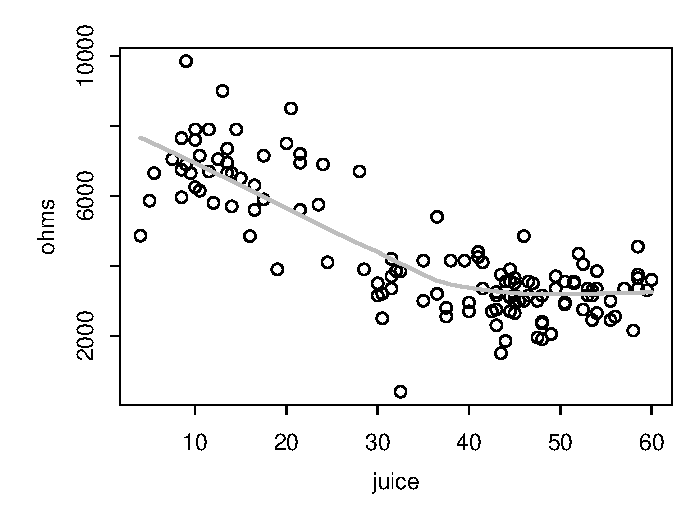
\includegraphics[width=0.65\textwidth]{figs/xmeth-smooth-ohms-12_1-1} 

}



\end{knitrout}
  \caption{Resistance in ohms is plotted against apparent juice
    content.  A smooth curve (in gray) has been added, using the
    \txtt{lowess} smoother.  The width of the smoothing window was the
    default fraction $f = \frac{2}{3}$ of the range of values of the
    $x$-variable.}\label{fig:fruitohms}
\end{figure}

\begin{figure}
\begin{knitrout}
\definecolor{shadecolor}{rgb}{0.969, 0.969, 0.969}\color{fgcolor}

{\centering 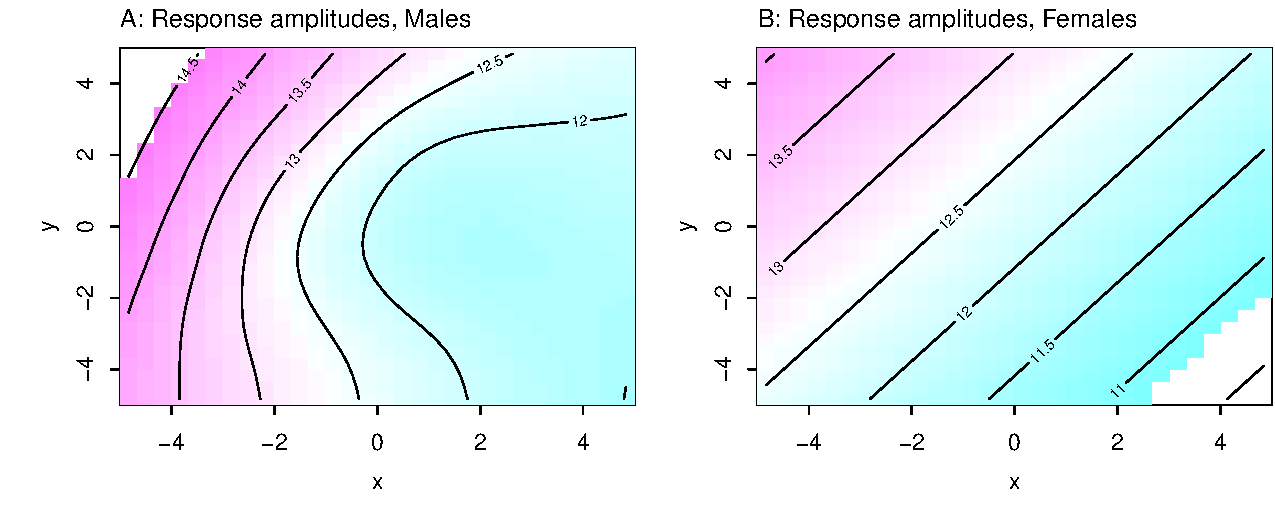
\includegraphics[width=0.97\textwidth]{figs/xmeth-plotVIS-12_2-1} 

}



\end{knitrout}
\caption{Estimated contours of left eye responses to visual stimulae,
projected onto the plane.\label{fig:visAmp}}
\end{figure}

\begin{figure}
\begin{knitrout}
\definecolor{shadecolor}{rgb}{0.969, 0.969, 0.969}\color{fgcolor}

{\centering 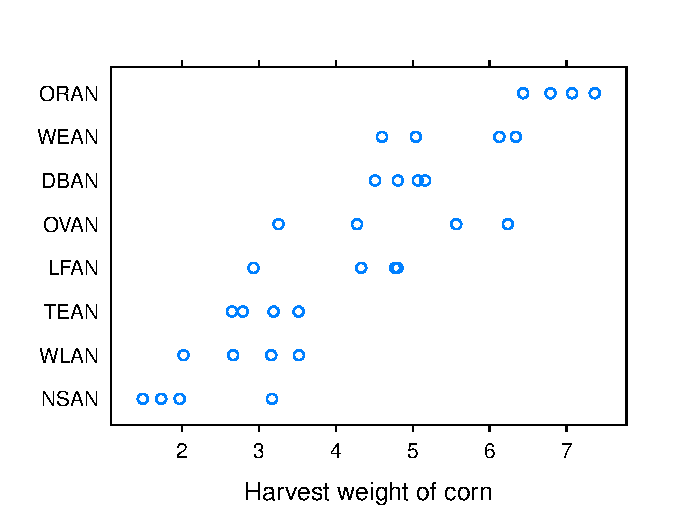
\includegraphics[width=0.65\textwidth]{figs/xmeth-ant111b-12_3-1} 

}



\end{knitrout}
\caption{Yields from 4 packages of land on each of eight sites on the
  Caribbean island of Antigua. Data are a summarized version of a
  subset of data given in Andrews and Herzberg 1985,
  pp.\~339-353.\label{fig:caribbean}}
\end{figure}

\begin{knitrout}
\definecolor{shadecolor}{rgb}{0.969, 0.969, 0.969}\color{fgcolor}\begin{kframe}
\begin{alltt}
\hlcom{## ---- getErie ----}
\hlstd{Erie} \hlkwb{<-} \hlstd{greatLakes[,}\hlstr{"Erie"}\hlstd{]}
\end{alltt}
\end{kframe}
\end{knitrout}

\begin{figure}
\begin{knitrout}
\definecolor{shadecolor}{rgb}{0.969, 0.969, 0.969}\color{fgcolor}

{\centering 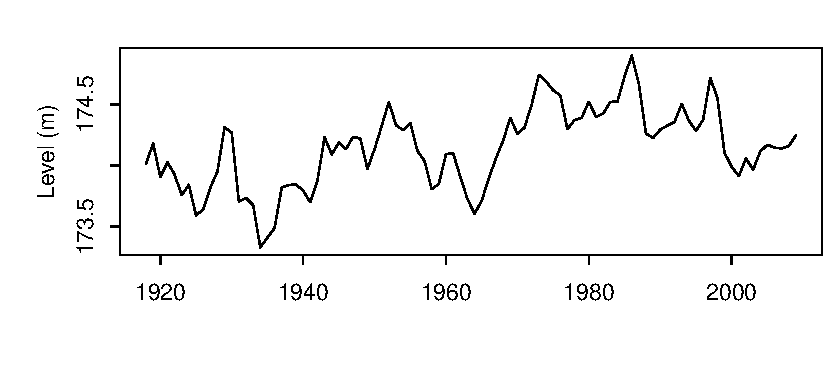
\includegraphics[width=0.8\textwidth]{figs/xmeth-Erie1-12_4-1} 

}



\end{knitrout}
\caption{Level of Lake Erie, in meters.
}\label{fig:erie}
\end{figure}

\begin{figure}
\begin{knitrout}
\definecolor{shadecolor}{rgb}{0.969, 0.969, 0.969}\color{fgcolor}

{\centering 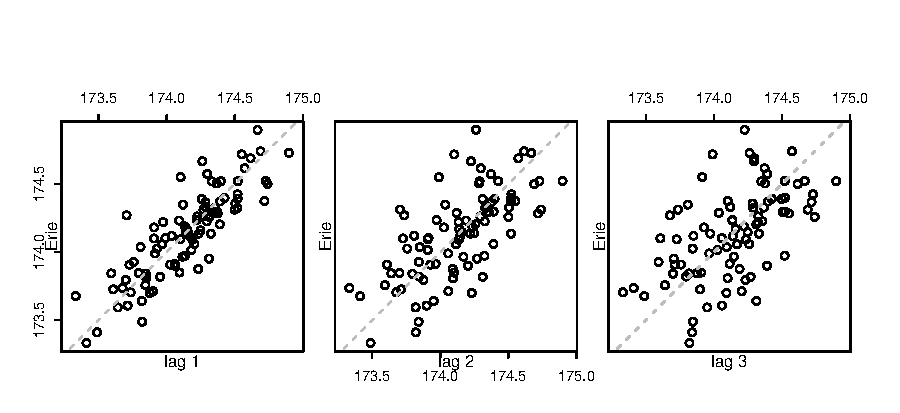
\includegraphics[width=0.98\textwidth]{figs/xmeth-lagErie-12_5-1} 

}



\end{knitrout}
\vspace*{-3pt}

\begin{knitrout}
\definecolor{shadecolor}{rgb}{0.969, 0.969, 0.969}\color{fgcolor}

{\centering 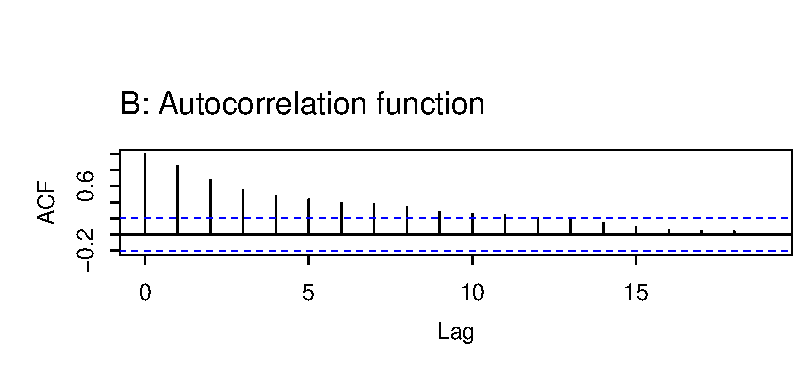
\includegraphics[width=0.7\textwidth]{figs/xmeth-acfErie-1} 

}



\end{knitrout}
\caption{Panel A plots Lake Erie levels vs levels at lags 1, 2 and 3
  respectively. Panel B shows a consistent pattern of decreasing
  autocorrelation at successive lags.
}\label{erie-lagplot}
\end{figure}

\begin{figure}
\begin{knitrout}
\definecolor{shadecolor}{rgb}{0.969, 0.969, 0.969}\color{fgcolor}

{\centering 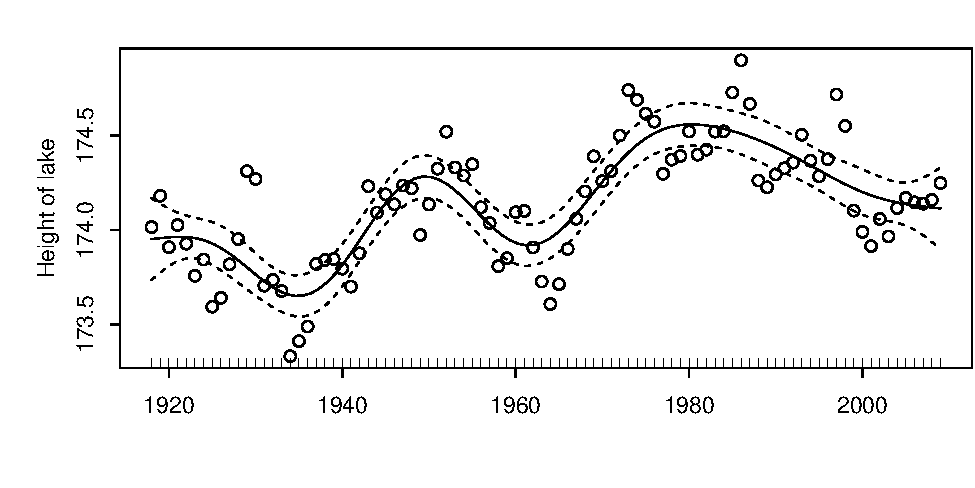
\includegraphics[width=0.75\textwidth]{figs/xmeth-gamErie-12_6-1} 

}



\end{knitrout}
\caption{GAM smoothing term, fitted to the Lake Erie Data.
    Most of the autocorrelation structure has been
    removed, leaving residuals that are very nearly independent.
  }\label{lh-smoothplot}
\end{figure}

\begin{figure}
\begin{knitrout}
\definecolor{shadecolor}{rgb}{0.969, 0.969, 0.969}\color{fgcolor}

{\centering 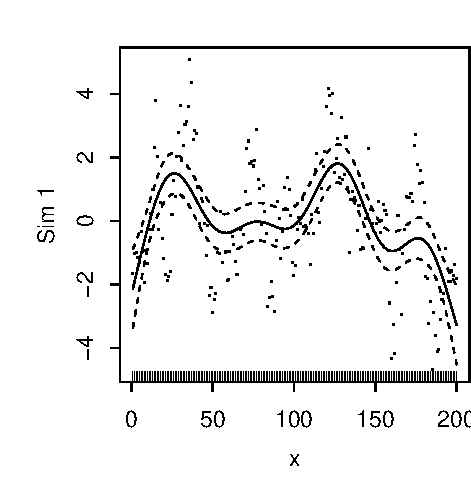
\includegraphics[width=0.32\textwidth]{figs/xmeth-arima-sim-12_7-1} 
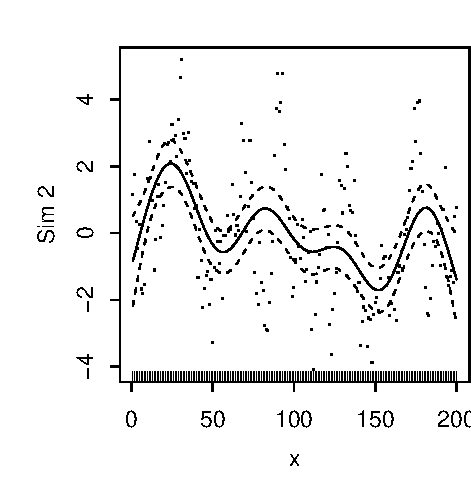
\includegraphics[width=0.32\textwidth]{figs/xmeth-arima-sim-12_7-2} 
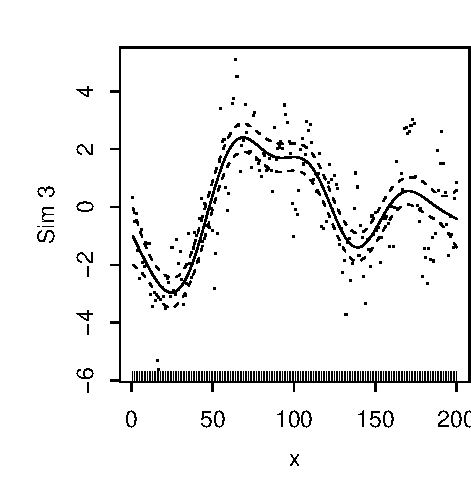
\includegraphics[width=0.32\textwidth]{figs/xmeth-arima-sim-12_7-3} 
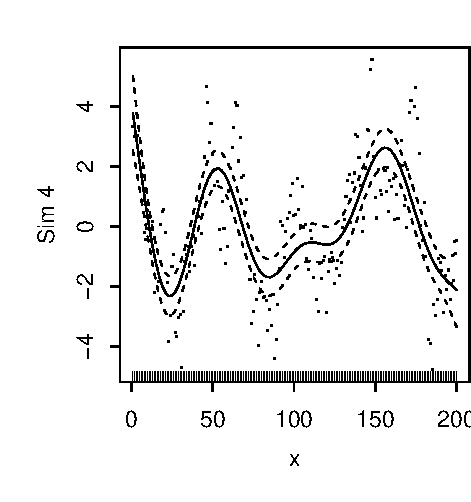
\includegraphics[width=0.32\textwidth]{figs/xmeth-arima-sim-12_7-4} 
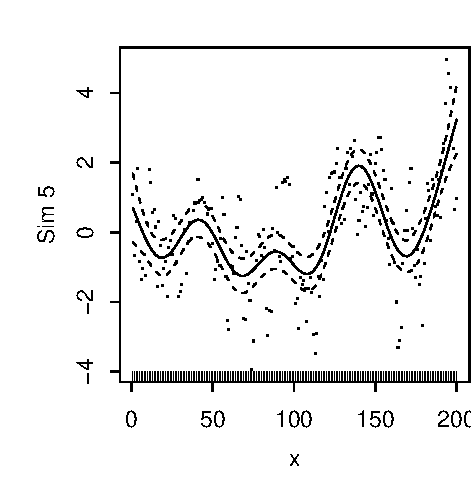
\includegraphics[width=0.32\textwidth]{figs/xmeth-arima-sim-12_7-5} 
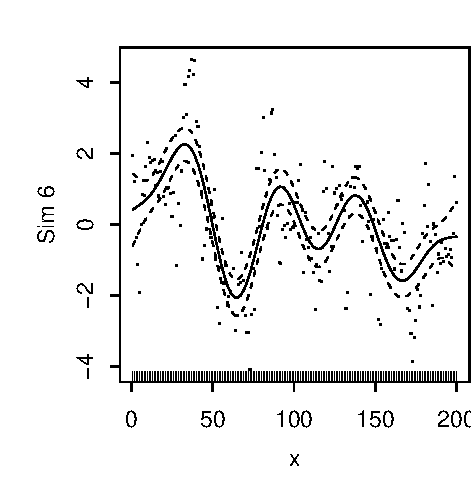
\includegraphics[width=0.32\textwidth]{figs/xmeth-arima-sim-12_7-6} 

}



\end{knitrout}
\caption{The plots are from repeated simulations of an AR1 process with a
  lag 1 correlation of 0.85.  Smooth curves, assuming independent
  errors, have been fitted.}\label{fig:ar1fits}
\end{figure}

\begin{figure}
\begin{knitrout}
\definecolor{shadecolor}{rgb}{0.969, 0.969, 0.969}\color{fgcolor}

{\centering 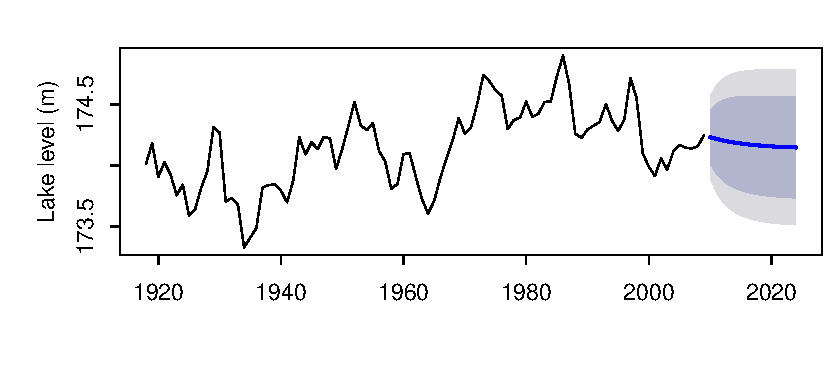
\includegraphics[width=0.8\textwidth]{figs/xmeth-Erie-fcast-12_8-1} 

}



\end{knitrout}
\caption{Predictions, 15 years into the future, of lake levels
  (m). The shaded areas give 80\% and 95\% confidence bounds.
}\label{Erie-fcastplot}
\end{figure}

\begin{figure}
\begin{knitrout}
\definecolor{shadecolor}{rgb}{0.969, 0.969, 0.969}\color{fgcolor}

{\centering 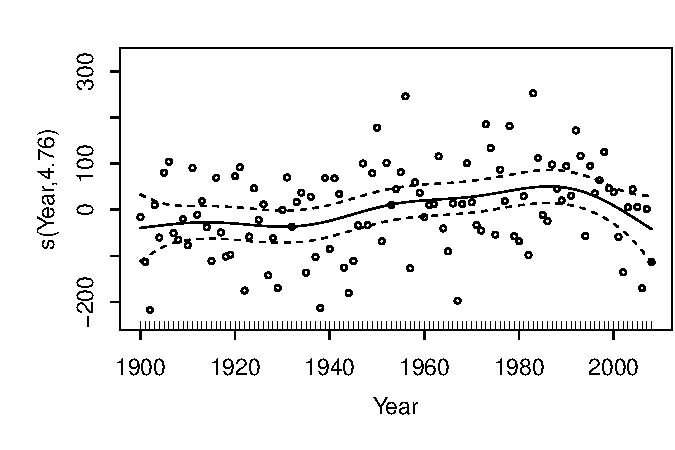
\includegraphics[width=0.47\textwidth]{figs/xmeth-mdb-gam-12_9-1} 
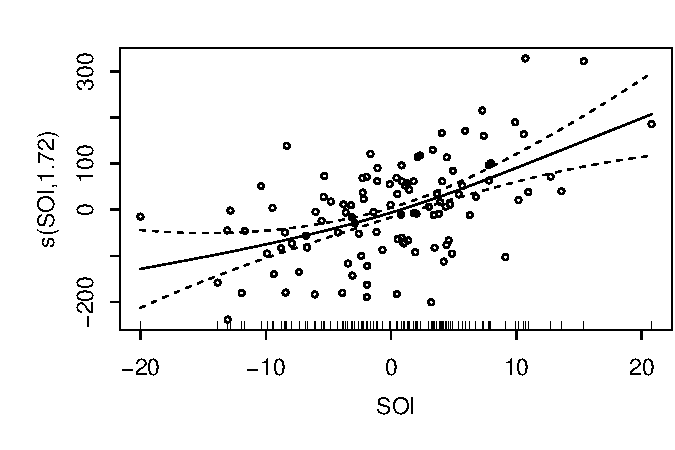
\includegraphics[width=0.47\textwidth]{figs/xmeth-mdb-gam-12_9-2} 

}



\end{knitrout}
  \caption{Estimated contributions of the model terms to
    \txtt{mdbRain}, in a GAM model that is the sum of smooth terms in
    \txtt{Year} and \txtt{Rain}. The dashed curves show pointwise
    2-SE limits, for the fitted curve.  Note the downturn
in the trend of \txtt{mdbRain} after about 1985,}\label{fig:mdbRainSM}
\end{figure}

\begin{figure}
\begin{knitrout}
\definecolor{shadecolor}{rgb}{0.969, 0.969, 0.969}\color{fgcolor}

{\centering 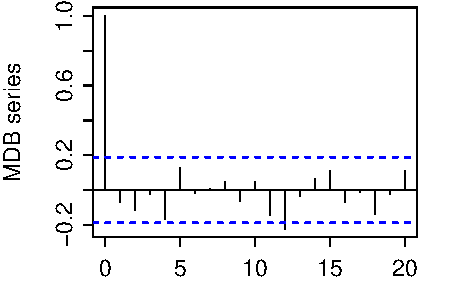
\includegraphics[width=0.32\textwidth]{figs/xmeth-ar1sims-12_10-1} 
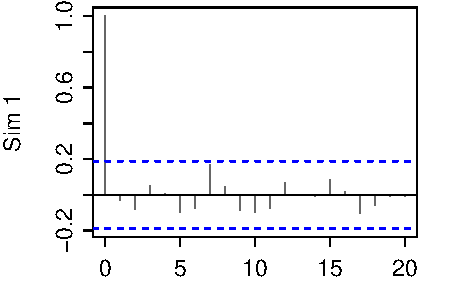
\includegraphics[width=0.32\textwidth]{figs/xmeth-ar1sims-12_10-2} 
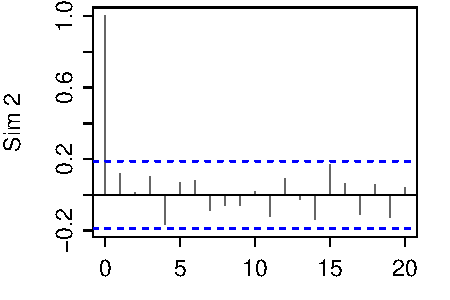
\includegraphics[width=0.32\textwidth]{figs/xmeth-ar1sims-12_10-3} 
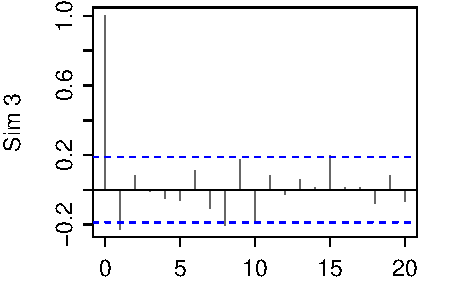
\includegraphics[width=0.32\textwidth]{figs/xmeth-ar1sims-12_10-4} 
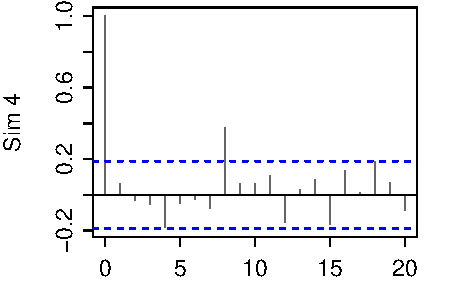
\includegraphics[width=0.32\textwidth]{figs/xmeth-ar1sims-12_10-5} 
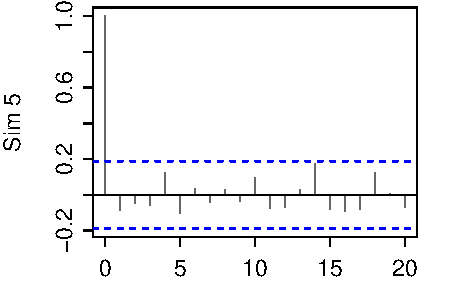
\includegraphics[width=0.32\textwidth]{figs/xmeth-ar1sims-12_10-6} 

}



\end{knitrout}
\caption{The top left panel shows the autocorrelation plot of the
  residuals from the GAM model \txtt{mdbRain.gam}.  The five remaining
  panels show autocorrelation plots for a series of independent random
  normal numbers.}\label{fig:ar1sims}
\end{figure}

\begin{figure*}[h]
\begin{knitrout}
\definecolor{shadecolor}{rgb}{0.969, 0.969, 0.969}\color{fgcolor}\begin{kframe}
\begin{verbatim}
[1] "Unable to plot graph. Ensure package 'gamclass' is installed."
NULL
\end{verbatim}
\end{kframe}

{\centering 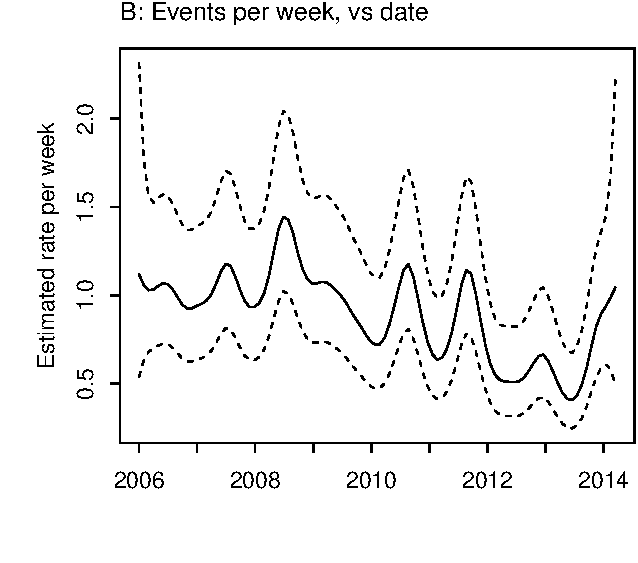
\includegraphics[width=0.47\textwidth]{figs/xmeth-au-both-12_11-1} 

}



\end{knitrout}
\caption{Estimated number of events (aircraft crashes) per time
  interval versus time.  In Panel A, the outcome variable was events
  per day, while in Panel B it was events per
  week.\label{fig:planeCrash}}
\end{figure*}

\begin{figure}
\begin{knitrout}
\definecolor{shadecolor}{rgb}{0.969, 0.969, 0.969}\color{fgcolor}

{\centering 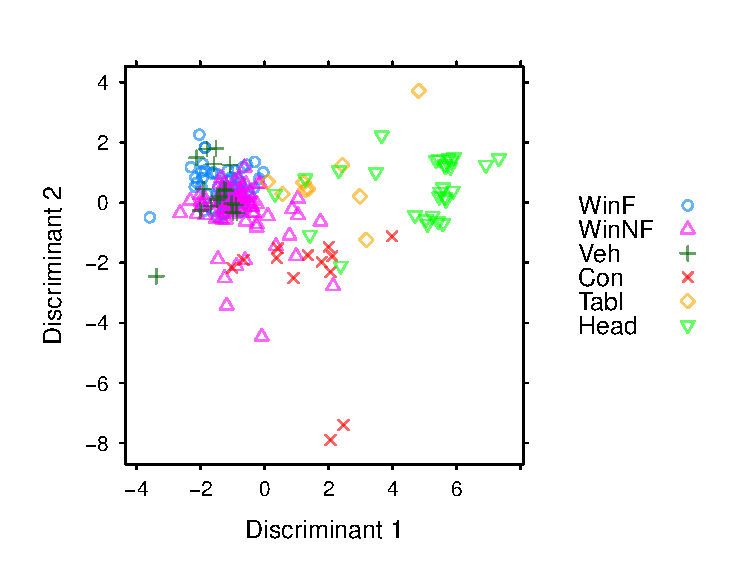
\includegraphics[width=0.65\textwidth]{figs/xmeth-fgl-scores2D-12_12-1} 

}



\end{knitrout}
\caption{Visual representation of a classification rule, derived using
  {\em linear discriminant analysis}, for the forensic glass data.  A
  five-dimensional pattern of separation between the categories has
  been collapsed down to two dimensions.  Some categories may therefore
be better distinguished than is evident from this figure.
}
\label{fig:fgl}
\end{figure}

\begin{knitrout}
\definecolor{shadecolor}{rgb}{0.969, 0.969, 0.969}\color{fgcolor}\begin{kframe}
\begin{alltt}
\hlkwd{library}\hlstd{(rpart,} \hlkwc{quietly}\hlstd{=}\hlnum{TRUE}\hlstd{)}
\end{alltt}
\end{kframe}
\end{knitrout}

\begin{figure}
\begin{knitrout}
\definecolor{shadecolor}{rgb}{0.969, 0.969, 0.969}\color{fgcolor}

{\centering 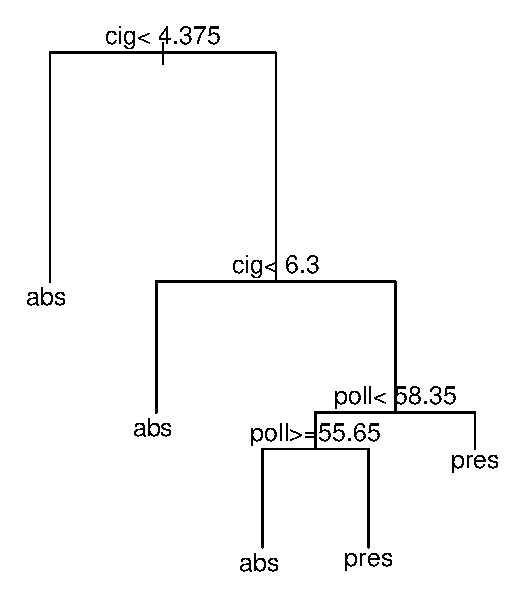
\includegraphics[width=0.55\textwidth]{figs/xmeth-treefig-12_13-1} 

}



\end{knitrout}
\caption{Decision tree for predicting whether a miner has
    bronchitis.  Where the condition at a node is satisfied, the left
    branch is taken. Thus, at the initial node, \txtt{cig$<$4.385}
    takes the branch to the left.  In general, unless a random number
    seed is specified, the tree may be different for each different run of the
    calculations.
}\label{fig:tree}
\end{figure}

\begin{figure}
\begin{knitrout}
\definecolor{shadecolor}{rgb}{0.969, 0.969, 0.969}\color{fgcolor}

{\centering 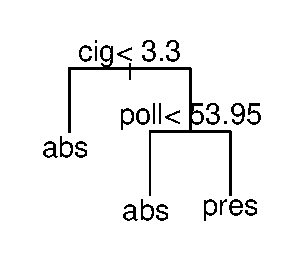
\includegraphics[width=0.24\textwidth]{figs/xmeth-rf-x-bronchit-1} 
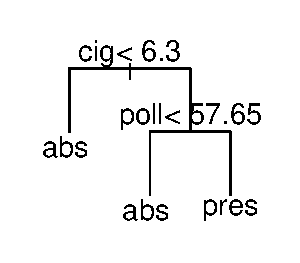
\includegraphics[width=0.24\textwidth]{figs/xmeth-rf-x-bronchit-2} 
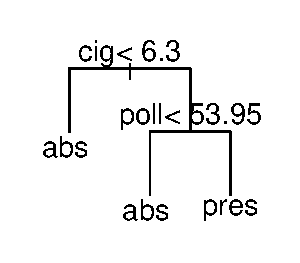
\includegraphics[width=0.24\textwidth]{figs/xmeth-rf-x-bronchit-3} 
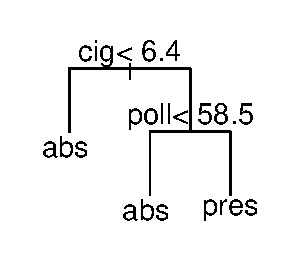
\includegraphics[width=0.24\textwidth]{figs/xmeth-rf-x-bronchit-4} 
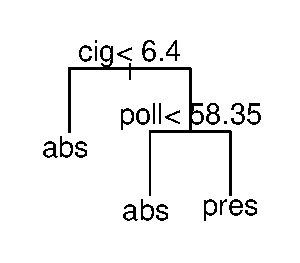
\includegraphics[width=0.24\textwidth]{figs/xmeth-rf-x-bronchit-5} 
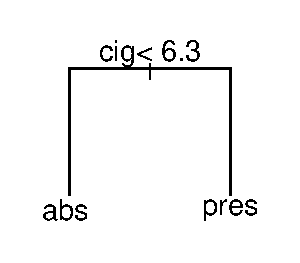
\includegraphics[width=0.24\textwidth]{figs/xmeth-rf-x-bronchit-6} 
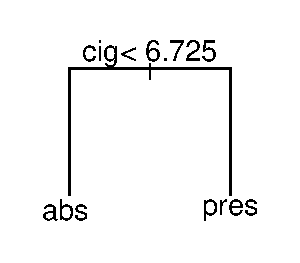
\includegraphics[width=0.24\textwidth]{figs/xmeth-rf-x-bronchit-7} 
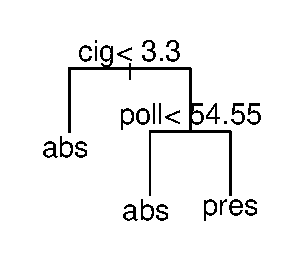
\includegraphics[width=0.24\textwidth]{figs/xmeth-rf-x-bronchit-8} 
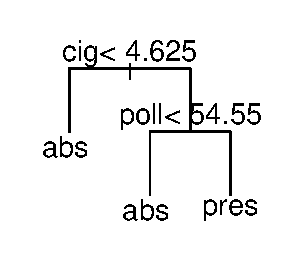
\includegraphics[width=0.24\textwidth]{figs/xmeth-rf-x-bronchit-9} 
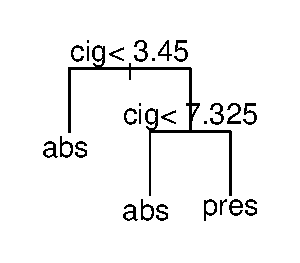
\includegraphics[width=0.24\textwidth]{figs/xmeth-rf-x-bronchit-10} 
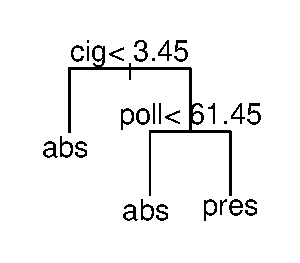
\includegraphics[width=0.24\textwidth]{figs/xmeth-rf-x-bronchit-11} 
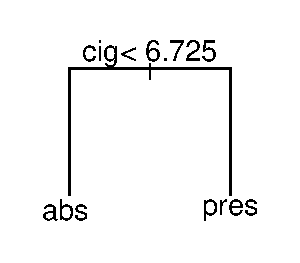
\includegraphics[width=0.24\textwidth]{figs/xmeth-rf-x-bronchit-12} 

}



\end{knitrout}
\caption{Each tree is for a different bootstrap sample of
  observations.  The final classification is determined by a random
  vote over all trees.  Where there are $>$ 2 explanatory variables
  (but not here) a different random sample of variables is typically
  used for each different split. The final classification is
  determined by a random vote over all trees.}\label{fig:brontrees}
\end{figure}

\begin{figure}
\begin{knitrout}
\definecolor{shadecolor}{rgb}{0.969, 0.969, 0.969}\color{fgcolor}

{\centering 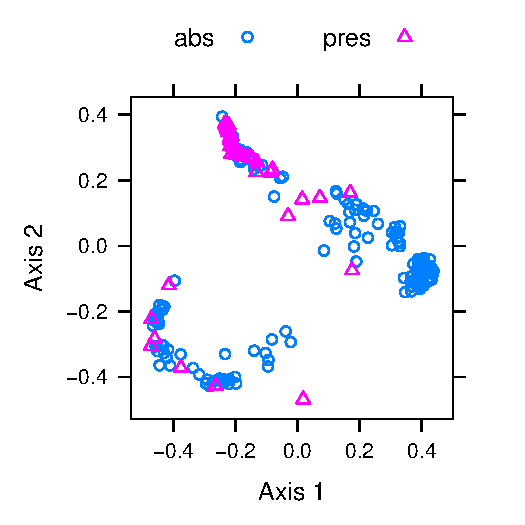
\includegraphics[width=0.47\textwidth]{figs/xmeth-proximity-plot-1} 

}



\end{knitrout}
\caption{The plot is designed to represent, in two dimensions, the random
  forest result. It aims to reflect probabilities of group membership
  given by the analysis.  It is not derived by a 'scaling' of the
  feature space.
}\label{fig:rfbronchit}
\end{figure}
%$

\begin{knitrout}
\definecolor{shadecolor}{rgb}{0.969, 0.969, 0.969}\color{fgcolor}\begin{kframe}
\begin{alltt}
\hlcom{## ---- aupoints ----}
\hlstd{aupts} \hlkwb{<-} \hlkwd{cmdscale}\hlstd{(audists)}
\end{alltt}
\end{kframe}
\end{knitrout}

\begin{figure}
\begin{knitrout}
\definecolor{shadecolor}{rgb}{0.969, 0.969, 0.969}\color{fgcolor}

{\centering 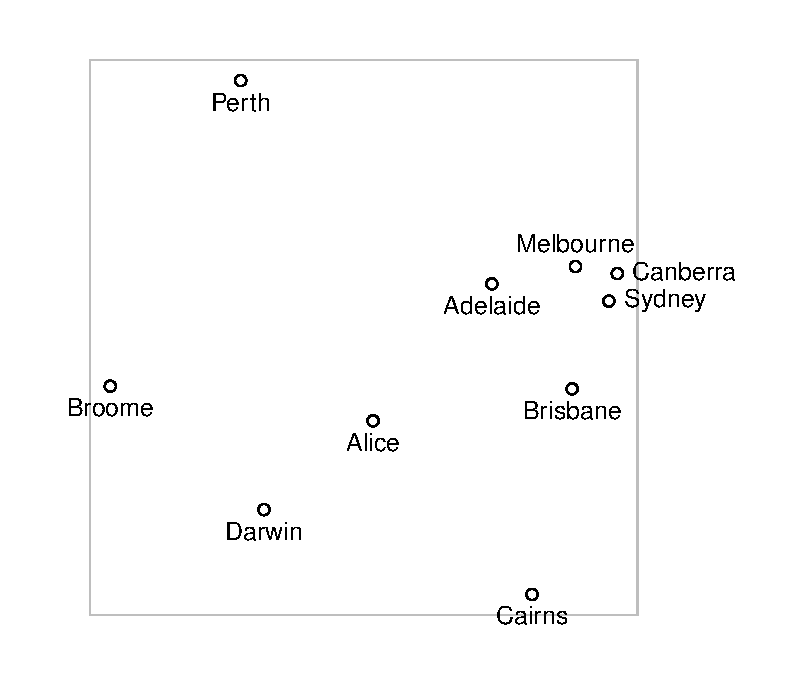
\includegraphics[width=0.6\textwidth]{figs/xmeth-aupoints_12_16-1} 

}



\end{knitrout}
\caption{Relative locations of Australian cities, derived from road
  map distances, using metric scaling.\label{fig:audists}}
\end{figure}



\begin{figure*}[h]
\begin{knitrout}
\definecolor{shadecolor}{rgb}{0.969, 0.969, 0.969}\color{fgcolor}

{\centering 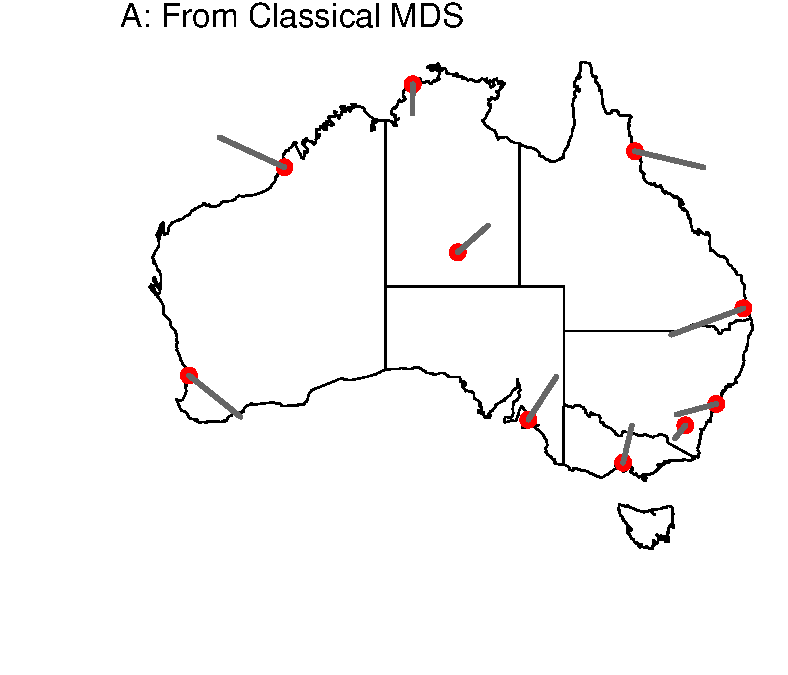
\includegraphics[width=0.47\textwidth]{figs/xmeth-au-both-12_17-1} 
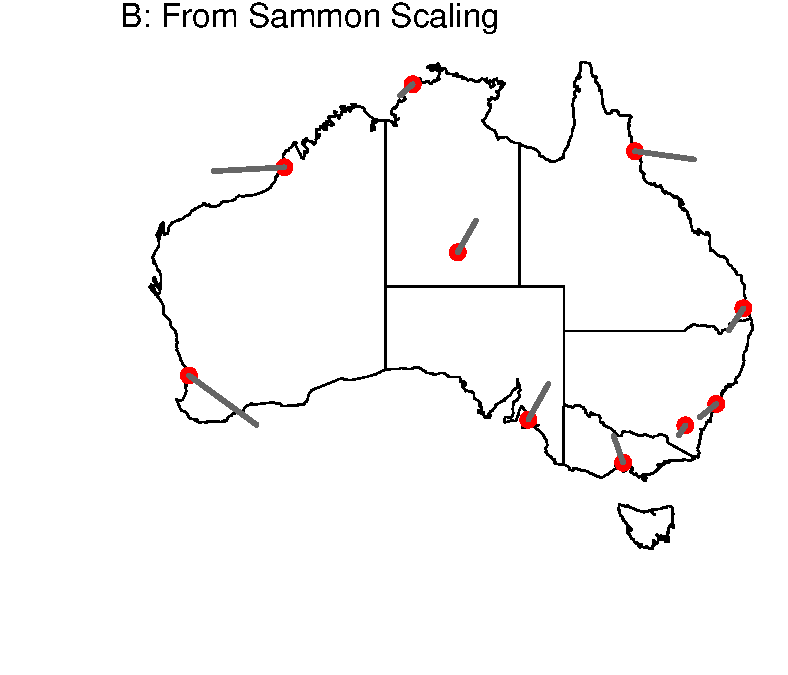
\includegraphics[width=0.47\textwidth]{figs/xmeth-au-both-12_17-2} 

}



\end{knitrout}
      \caption{In Panel A, Figure \ref{fig:audists} has been rotated and
        scaled, to give a best fit to a map of Australia.  Each city
        moves as shown by the line that radiates out from it.  Panel B
        is the equivalent plot for the Sammon scaling ordination.
\label{fig:aufit}}
\end{figure*}

\end{document}


